\chapter{Kodierung und empirische Analyse von bedingter Unabhängigkeit der stable, complete und preferred Semantik}
\label{ch:semantic-independence}


Hier ein großer Ausblick, was alles im Kapitel passiert. Bereits zitieren, wer was gemacht hat und worauf wir aufbauen.

Die semantische Definition geht auf
\textcite{rienstra:2020:independence-af} zurück. Notation und
Komplexitätsergebnisse orientieren sich an
\textcite{bluemel:2025:independence-aba}. QBFs als Zielformalismus für
Argumentationsprobleme wurden insbesondere von
\textcite{egly:woltran:2006:reasoning-qbf} untersucht.

\section{Sektion 1: Entscheidungsproblen \& Komplexität}
\label{sec:sigma-independence-af-complexity}

\iffalse
Eine Semantik ordnet einem Argumentationssystem im Allgemeinen mehrere
zulässige Labellings zu. Dadurch können die Bewertungen verschiedener
Argumentmengen miteinander verknüpft sein. Wird etwa das Label eines
Arguments aus \(X\) festgelegt, kann dies die möglichen Labels der
Argumente aus \(Y\) einschränken.

Semantikspezifische Unabhängigkeit liegt vor, wenn solche Einschränkungen
nach Fixierung der Labels auf einer Konditionierungsmenge \(Z\) nicht
auftreten. Dazu werden zwei zulässige Labellings betrachtet, die auf
\(Z\) übereinstimmen. Die Bewertung von \(X\) aus dem ersten und die
Bewertung von \(Y\) aus dem zweiten Labelling müssen sich dann zu einem
weiteren zulässigen Labelling kombinieren lassen.



Die Definition lässt sich damit als Abschlussbedingung der Menge der
\(\sigma\)-Labellings unter partieller Kombination verstehen. Zum
Nachweis der Abhängigkeit genügt es, zwei \(\sigma\)-Labellings
\(\lambda_1\) und \(\lambda_2\) anzugeben, die auf \(Z\) übereinstimmen,
deren Bewertungen auf \(X\) beziehungsweise \(Y\) sich aber durch kein
\(\sigma\)-Labelling kombinieren lassen.

Die semantische Definition beschreibt eine Eigenschaft eines festen
Argumentationssystems. Im Folgenden wird die algorithmische Aufgabe
betrachtet, diese Eigenschaft für eine gegebene Instanz zu entscheiden.
\fi

\begin{Definition}[\cite{bluemel:2025:independence-aba}]
    \label{def:sigma-independence-af-dec-problem}
    Für \(\sigma\in\{\mathsf{co},\mathsf{st},\mathsf{pr}\}\) bezeichnet
    \(\mathrm{IND}_\sigma\) das folgende \emph{Entscheidungsproblem}:
    \[
        \begin{array}{ll}
        \text{Eingabe:}
            &AF~F =(A,R)\text{ sowie paarweise disjunkte Mengen }
             X,Y,Z\subseteq A\\
        \text{Frage:}
            &\text{Gilt }X\perp_\sigma Y\mid Z\text{ in }F\,?
        \end{array}
    \]
    Für \(x,y\in A\) stehen
    \(x\perp_\sigma y\mid Z\) und
    \(x\not\perp_\sigma y\mid Z\) kurz für die entsprechenden Aussagen
    über die Singletonmengen \(\{x\}\) und \(\{y\}\).
\end{Definition}


Die Entscheidungsprobleme zur semantikspezifischen Unabhängigkeit weisen
bereits für die betrachteten Standardsemantiken eine hohe Komplexität auf.

\begin{Theorem}[\cite{bluemel:2025:independence-aba}]
\label{thm:independence-complexity}
Die Entscheidungsprobleme
\(\mathrm{IND}_{\mathsf{co}}\) und
\(\mathrm{IND}_{\mathsf{st}}\) sind
\(\Pi^{\mathrm P}_2\)-vollständig.
Das Entscheidungsproblem
\(\mathrm{IND}_{\mathsf{pr}}\) ist
\(\Pi^{\mathrm P}_3\)-vollständig.
\end{Theorem}

Die Vollständigkeitsergebnisse motivieren QBFs als Zielformalismus:
QBFs mit zwei beziehungsweise drei alternierenden Quantorenblöcken
erfassen genau die relevanten Stufen der polynomiellen Hierarchie. Bevor
die Quantorenstruktur der Unabhängigkeit formuliert werden kann, müssen
zunächst einzelne Labellings und ihre semantische Gültigkeit
aussagenlogisch kodiert werden.

Eine besondere Rolle nehmen AFs ein, die über kein oder nur ein Labelling verfügen.

\begin{Lemma}
    \label{lem:independence-trivial-labelling-set}
    Gilt \(|\Lambda_\sigma(F)|\leq 1\), so gilt
    \(X\perp_\sigma Y\mid Z\) für alle paarweise disjunkten Mengen
    \(X,Y,Z\subseteq A\).
\end{Lemma}

\begin{proof}
    Für \(\Lambda_\sigma(F)=\emptyset\) ist die Allquantifizierung über
    \(\lambda_1\) und \(\lambda_2\) leer. Besteht
    \(\Lambda_\sigma(F)\) aus genau einem Labelling \(\lambda\), so kann
    für das einzige Paar \((\lambda,\lambda)\) dieses Labelling selbst als
    \(\lambda_3\) gewählt werden.
\end{proof}

Das Lemma ist für die spätere empirische Auswertung wesentlich: Eine hohe
Unabhängigkeitsrate kann sowohl durch viele Kombinationsmöglichkeiten als auch durch
das Fehlen vergleichbarer Labellings entstehen.

\section{Kodierung der stable, complete und preferred Semantik}
\label{sec:semantics-encoding}

ROADMAP:
Kodierung der Semantiken: stable, complete, preferred, um anschließend QBF aufzustellen
Zuerst Hilfvariablen, die Labelling induzieren
dann Semantiken kodieren
dann Kodierung nutzen, um QBF für sigma-Unabhängigkeit aufzustellen

KURZE BESCHREIBUNG, WAS PASSIEREN WIRD

\begin{Definition}
    \label{def:labelling-variable-block}
    Sei \(F=(A,R)\) ein Argumentationssystem. Ein
    \emph{Labellingvariablenblock} für \(F\) ist ein Tripel
    \(\mathbf{V}=(I,O,U)\) paarweise disjunkter Variablenmengen
\(
        I=\{i_a\mid a\in A\},~
        O=\{o_a\mid a\in A\},~
        U=\{u_a\mid a\in A\}.
\)
\end{Definition}
Die Variablen \(i_a\), \(o_a\) und \(u_a\) kodieren die Labels
\(\mathsf{in}\), \(\mathsf{out}\) beziehungsweise \(\mathsf{und}\)
von \(a\). 

\begin{Definition}
    Sei \(\mathbf V =(I,O,U)\) ein Labellingsvariablenblock. Wir definieren:
    \[
    \operatorname{One}_F(\mathbf V)
    :=
    \bigwedge_{a\in A}
    \Bigl(
        (i_a\lor o_a\lor u_a)
        \land\neg(i_a\land o_a)
        \land\neg(i_a\land u_a)
        \land\neg(o_a\land u_a)
    \Bigr).
\]
\end{Definition}
Die Formel \(\operatorname{One}_F(\mathbf V)\)
garantiert, dass in der Repräsentation jedes Argument genau ein Label trägt. 


WIE MACHEN? LEMMA, DASS One EIN LABELLING induziert
\begin{Definition}
    Jede Belegung \(\nu\models\operatorname{One}_F(\mathbf V)\)
    induziert das \emph{kodierte Labelling} \(\lambda_\nu\) durch
    \[
        \lambda_\nu(a)=
        \begin{cases}
            \mathsf{in},  &\text{falls }\nu(i_a)=1,\\
            \mathsf{out}, &\text{falls }\nu(o_a)=1,\\
            \mathsf{und}, &\text{falls }\nu(u_a)=1.
        \end{cases}
    \]
\end{Definition}
Mit \(\mathbf V^k=(I^k,O^k,U^k)\) bezeichnen wir eine
\emph{\(k\)-te Kopie} dieses Blocks, deren Variablen mit dem
Superskript \(k\) versehen werden. 

DIESE AUSSAGE als LEMMA und BEWEISEN
Damit besteht eine Bijektion zwischen den Labellings von \(F\) und den
Belegungen, die \(\operatorname{One}_F(\mathbf V)\) erfüllen: Jedes
Labelling bestimmt genau eine solche Belegung, und jede solche Belegung
bestimmt genau ein Labelling.


Vollständige Labellings lassen sich durch lokale Bedingungen
charakterisieren. Ein Argument erhält genau dann das Label
\(\mathsf{in}\), wenn alle seine Angreifer mit \(\mathsf{out}\)
markiert sind, und genau dann das Label \(\mathsf{out}\), wenn mindestens
ein Angreifer mit \(\mathsf{in}\) markiert ist. Stabile Labellings sind
die vollständigen Labellings, in denen das Label \(\mathsf{und}\) nicht
vorkommt.
\begin{Definition}
    \label{def:co-st-encodings}
    Sei \(F=(A,R)\) ein Argumentationssystem und
    \(\mathbf V=(I,O,U)\) ein Labellingvariablenblock. Wir definieren:
    \[
        \operatorname{Co}_F(\mathbf V)
        :=
        \operatorname{One}_F(\mathbf V)
        \land
        \bigwedge_{a\in A}
        \left(
            i_a\leftrightarrow
            \bigwedge_{b\in a^-}o_b
        \right)
        \land
        \bigwedge_{a\in A}
        \left(
            o_a\leftrightarrow
            \bigvee_{b\in a^-}i_b
        \right).
    \]
\end{Definition}
HIER BESCHREIBUNG DER FORMEL UND ERKLÄRUNG, WARUM KORREKT
\begin{Definition}
    Sei \(F=(A,R)\) ein Argumentationssystem und
    \(\mathbf V=(I,O,U)\) ein Labellingvariablenblock. Wir definieren:
    \[
        \operatorname{St}_F(\mathbf V)
        :=
        \operatorname{Co}_F(\mathbf V)
        \land
        \bigwedge_{a\in A}\neg u_a.
    \]
\end{Definition}
HIER BESCHREIBUNG DER FORMEL UND ERKLÄRUNG, WARUM KORREKT

Während Complete und Stable durch Bedingungen innerhalb eines einzelnen
Labellings charakterisiert werden können, vergleicht die
Preferred-Semantik ein vollständiges Labelling mit allen anderen
vollständigen Labellings. Dafür wird eine zweite Kopie des
Variablenblocks benötigt.
\begin{Definition}[\cite{egly:woltran:2006:reasoning-qbf}]
    \label{def:strict-inclusion}
    Seien \(\mathbf V=(I,O,U)\) und
    \(\widehat{\mathbf V}=(\widehat{I},\widehat{O},\widehat{U})\) zwei Labellingvariablenblöcke für das 
    \(AF ~F=(A,R)\). Wir definieren:
    \[
        I < \widehat{I}
        :=
        \left(
            \bigwedge_{a\in A}(i_a\rightarrow \widehat{i_a})
        \right)
        \land
        \left(
            \bigvee_{a\in A}(\neg i_a\land \widehat{i_a})
        \right).
    \]
\end{Definition}
Die Formel ist genau dann erfüllt, wenn \(\mathbf V\) ein vollständiges
Labelling kodiert und kein vollständiges Labelling mit echt größerer
In-Menge existiert. Die Vergleichsvariablen
\(\widehat{\mathbf V}\) sind dabei bei jeder Verwendung der Formel
frisch zu wählen.
\begin{Definition}
    \label{def:preferred-encoding}
    Seien \(\mathbf V, \widehat{\mathbf V}\) Labellingvariablenblöcke. Wir definieren:
    \[
        \operatorname{Pr}_F(\mathbf V)
        :=
        \operatorname{Co}_F(\mathbf V)
        \land
        \forall\widehat{\mathbf V}\,
        \neg ({Co}_F(\widehat{\mathbf V})
        \land I < \widehat{I}).
    \]
\end{Definition}
HIER BESCHREIBUNG DER FORMEL UND ERKLÄRUNG, WARUM KORREKT
\begin{Definition}
    \label{def:uniform-semantics-predicate}
    Für
    \(\sigma\in\{\mathsf{co},\mathsf{st},\mathsf{pr}\}\) definieren wir:
    \[
        \operatorname{Sem}^{\sigma}_F(\mathbf V)
        :=
        \begin{cases}
            \operatorname{Co}_F(\mathbf V),
                &\text{falls }\sigma=\mathsf{co},\\
            \operatorname{St}_F(\mathbf V),
                &\text{falls }\sigma=\mathsf{st},\\
            \operatorname{Pr}_F(\mathbf V),
                &\text{falls }\sigma=\mathsf{pr}.
        \end{cases}
    \]
\end{Definition}
HIER BESCHREIBUNG DER FORMEL.
\begin{Lemma}
    \label{lem:semantics-encoding-correct}
    Sei \(\nu\models\operatorname{One}_F(\mathbf V)\), und sei
    \(\lambda_\nu\) das durch \(\nu\) kodierte Labelling. Für jedes
    \(\sigma\in\{\mathsf{co},\mathsf{st},\mathsf{pr}\}\) gilt
    \[
        \nu\models\operatorname{Sem}^{\sigma}_F(\mathbf V)
        \quad\Longleftrightarrow\quad
        \lambda_\nu\in\Lambda_\sigma(F).
    \]
\end{Lemma}
\begin{proof}
    Für \(\sigma=\mathsf{co}\) geben die beiden Äquivalenzen in
    \(\operatorname{Co}_F\) genau die Definition eines vollständigen
    Labellings wieder. Für \(\sigma=\mathsf{st}\) kommt die Bedingung
    \(\mathsf{und}(\lambda_\nu)=\emptyset\) hinzu.

    Für \(\sigma=\mathsf{pr}\) ist
    \(\forall\widehat{\mathbf V}\,
        \neg ({Co}_F(\widehat{\mathbf V})
        \land I < \widehat{I})\) genau dann wahr, wenn kein vollständiges Labelling existiert,
    dessen In-Menge die In-Menge von \(\lambda_\nu\) echt enthält.
    Dies ist äquivalent zur In-Maximalität von \(\lambda_\nu\).
\end{proof}
Alle verwendeten Formeln besitzen eine Größe in
\(O(|A|+|R|)\).

\section{QBF-Kodierung der bedingten Unabhängigkeit}
\label{sec:uniform-independence-qbf}

HIER ROADMAP, WAS IN DIESER SECTION PASSIERT.
Die Definition der Unabhängigkeit benötigt drei Labellings. Ihre
Übereinstimmung auf ausgewählten Argumentmengen wird unabhängig von der
Semantik kodiert.

ERKLÄRUNG MIT SUPERSKRIPT UND LABELLINGVRIABLENBLOCK.
\begin{Definition}
    \label{def:equality-and-mix-formulas}
    Sei \(F =(A,R)\) ein AF, \(S\subseteq A\) und seien\(\mathbf V^j\) und \(\mathbf V^k\) zwei Kopien des
    Labellingvariablenblocks. Wir definieren:
    \[
        \operatorname{Eq}^{j,k}_S
        :=
        \bigwedge_{a\in S}
        \Bigl(
            (i_a^j\leftrightarrow i_a^k)
            \land(o_a^j\leftrightarrow o_a^k)
            \land(u_a^j\leftrightarrow u_a^k)
        \Bigr).
    \]
\end{Definition}
WAS MACHT DAS, WOFÜR BRAUCHEN WIR ES?
\begin{Definition}

    Sei \(F =(A,R)\) ein AF und sei \(\operatorname{Eq}^{j,k}_S\) wie in \ref{def:equality-and-mix-formulas} definiert.
    Für paarweise disjunkte Mengen \(X,Y,Z\subseteq A\) definieren wir:
    \[
        \operatorname{Mix}^{1,2,3}_{X,Y\mid Z}
        :=
        \operatorname{Eq}^{1,3}_X
        \land
        \operatorname{Eq}^{2,3}_Y
        \land
        \operatorname{Eq}^{1,3}_Z
    \]
\end{Definition}
WAS MACHT DAS, WOFÜR BRAUCHEN WIR ES?
\begin{Lemma}
    \label{lem:equality-and-mix-correct}
    Kodieren die Blöcke \(\mathbf V^1,\mathbf V^2,\mathbf V^3\) die
    Labellings \(\lambda_1,\lambda_2,\lambda_3\), so gilt
    \(
        \operatorname{Eq}^{j,k}_S
        \Longleftrightarrow
        \lambda_j|_S=\lambda_k|_S
    \)
    und
    \(
        \operatorname{Mix}^{1,2,3}_{X,Y\mid Z}
        \Longleftrightarrow
        \left(
        \lambda_3|_X=\lambda_1|_X
        \land
        \lambda_3|_Y=\lambda_2|_Y
        \land
        \lambda_3|_Z=\lambda_1|_Z
        \right).
    \)
\end{Lemma}

\begin{proof}
    Aufgrund der Eindeutigkeit der Kodierung ist für jedes Argument genau eine der drei
    Labelvariablen wahr. Die drei Äquivalenzen für ein Argument sind daher
    genau dann erfüllt, wenn beide Blöcke dasselbe Label kodieren. Die zweite
    Aussage folgt durch Einsetzen der drei Gleichheitsformeln.
\end{proof}

Damit stehen sowohl die semantische Gültigkeit der drei Labellings als
auch ihre erforderlichen Übereinstimmungen als getrennte Bausteine zur
Verfügung. Diese können nun entsprechend der Quantorenstruktur der
Unabhängigkeitsdefinition zusammengesetzt werden.

Die beiden universellen Variablenblöcke repräsentieren die beliebig
gewählten Labellings \(\lambda_1\) und \(\lambda_2\). Der existentielle
Block repräsentiert das kombinierende Labelling \(\lambda_3\). Die
Prämisse der Implikation beschränkt die universellen Belegungen auf
\(\sigma\)-Labellings, die auf \(Z\) übereinstimmen.
\begin{Definition}
    \label{def:generic-independence-qbf}
    Sei \(F=(A,R)\) ein \(AF\), seien \(X,Y,Z\subseteq A\) paarweise disjunkt, seien \(\mathbf{V^1}, 
    \mathbf{V^2}, \mathbf{V^3}\) Labellingvariablenblöcke und sei
    \(\sigma\in\{\mathsf{co},\mathsf{st},\mathsf{pr}\}\). Die
    \emph{generische bedingte Unabhängigkeits-QBF} ist
    \[
    \begin{split}
        \Phi^\sigma_F(X,Y\mid Z)
        :=\forall\mathbf V^1\,\forall\mathbf V^2\,
        \Bigl(&
            \operatorname{Sem}^{\sigma}_F(\mathbf V^1)
            \land
            \operatorname{Sem}^{\sigma}_F(\mathbf V^2)
            \land
            \operatorname{Eq}^{1,2}_Z
        \\
        &\rightarrow
        \exists\mathbf V^3\,
        \bigl(
            \operatorname{Sem}^{\sigma}_F(\mathbf V^3)
            \land
            \operatorname{Mix}^{1,2,3}_{X,Y\mid Z}
        \bigr)
        \Bigr).
    \end{split}
    \]
    Bei der Preferred-Kodierung werden zusätzlich jeweils
    paarweise verschiedene Labellingvariablenblöcke
    \(\widehat{\mathbf V}^{1},
    \widehat{\mathbf V}^{2},
    \widehat{\mathbf V}^{3}\)
    verwendet.
\end{Definition}
WAS MACHT DIESE DEFINITION; WOFÜR BRAUCHT MAN SIE
\begin{Theorem}
    \label{thm:generic-independence-qbf-correct}
    Für jedes \(AF~F=(A,R)\), alle paarweise disjunkten Mengen
    \(X,Y,Z\subseteq A\) und jedes
    \(\sigma\in\{\mathsf{co},\mathsf{st},\mathsf{pr}\}\) gilt
    \[
        \Phi^\sigma_F(X,Y\mid Z)\text{ ist wahr}
        \quad\Longleftrightarrow\quad
        X\perp_\sigma Y\mid Z.
    \]
\end{Theorem}
\begin{proof}
    Sei die QBF wahr, und seien
    \(\lambda_1,\lambda_2\in\Lambda_\sigma(F)\) mit
    \(\lambda_1|_Z=\lambda_2|_Z\) gegeben. Ihre kodierenden Belegungen
    erfüllen nach Lemma~\ref{lem:semantics-encoding-correct} die beiden
    Semantikkodierungen und nach
    Lemma~\ref{lem:equality-and-mix-correct} die Formel
    \(\operatorname{Eq}^{1,2}_Z\). Die QBF liefert daher eine Belegung von
    \(\mathbf V^3\), die ein \(\sigma\)-Labelling \(\lambda_3\) kodiert
    und die geforderten Restriktionen erfüllt. Somit gilt
    \(X\perp_\sigma Y\mid Z\).

    Gelte umgekehrt \(X\perp_\sigma Y\mid Z\), und seien die beiden
    universellen Blöcke beliebig belegt. Ist die Prämisse falsch, ist die
    Implikation wahr. Andernfalls kodieren die Blöcke zwei
    \(\sigma\)-Labellings, die auf \(Z\) übereinstimmen. Nach Definition
    der Unabhängigkeit existiert ein passendes \(\lambda_3\). Seine
    kodierende Belegung erfüllt die Konklusion. Dies gilt für jede Belegung
    der universellen Blöcke, also ist die QBF wahr.
\end{proof}

\iffalse
\subsection{Quantorenstruktur der Spezialfälle}
\label{subsec:independence-prenex}

Für Complete und Stable sind die Semantikkodierungen quantorenfrei. Daher
kann der Existenzquantor für den dritten Block vor die Matrix gezogen
werden.

\begin{Proposition}
    \label{prop:co-st-independence-prenex}
    Für \(\sigma\in\{\mathsf{co},\mathsf{st}\}\) ist
    \(\Phi^\sigma_F(X,Y\mid Z)\) logisch äquivalent zu
    \[
    \begin{split}
        \forall\mathbf V^1\,\forall\mathbf V^2\,
        \exists\mathbf V^3\,
        \Bigl(&
        \bigl(
            \operatorname{Sem}^{\sigma}_F(\mathbf V^1)
            \land
            \operatorname{Sem}^{\sigma}_F(\mathbf V^2)
            \land
            \operatorname{Eq}^{1,2}_Z
        \bigr)
        \\
        &\rightarrow
        \bigl(
            \operatorname{Sem}^{\sigma}_F(\mathbf V^3)
            \land
            \operatorname{Mix}^{1,2,3}_{X,Y\mid Z}
        \bigr)
        \Bigr).
    \end{split}
    \]
    Die Formel besitzt damit zwei alternierende Quantorenblöcke.
\end{Proposition}

Bei Preferred dürfen die internen Quantoren der drei
Maximalitätsprüfungen nicht lediglich nebeneinandergestellt werden. Die
Maximalität der universell gewählten Labellings steht in der Prämisse und
kehrt deshalb beim Übergang in Negationsnormalform ihre Quantorenrichtung
um. Die folgende Formel macht diese Abhängigkeit explizit.

\begin{Definition}
    \label{def:preferred-independence-prenex}
    Für \(k\in\{1,2,3\}\) sei
    \(\widehat{\mathbf V}^{k}\) ein Labellingvariablenblock. Die
    \emph{pränexe Preferred-Unabhängigkeitskodierung} ist
    \[
    \begin{split}
        \Phi^{\mathsf{pr},\mathrm{PNF}}_F(X,Y\mid Z)
        := {}&
        \forall\mathbf V^1\,\forall\mathbf V^2\,
        \exists\mathbf V^3\,
        \exists\widehat{\mathbf V}^{1}\,
        \exists\widehat{\mathbf V}^{2}\,
        \forall\widehat{\mathbf V}^{3}
        \;\Bigl[
        \\
        &\neg\operatorname{Co}_F(\mathbf V^1)
        \lor
        \neg\operatorname{Co}_F(\mathbf V^2)
        \lor
        \neg\operatorname{Eq}^{1,2}_Z
        \\
        &\lor
        ({Co}_F(\widehat{\mathbf V}^{1})
        \land I^1 < I^1')
        \lor
        ({Co}_F(\widehat{\mathbf V}^{2})
        \land I^2 < I^2')
        \\
        &\lor
        \Bigl(
            \operatorname{Co}_F(\mathbf V^{3})
            \land
            \operatorname{Mix}^{1,2,3}_{X,Y\mid Z}
            \land
            \neg({Co}_F(\widehat{\mathbf V}^{3})
        \land I^3 < I^3')
        \Bigr)
        \Bigr].
    \end{split}
    \]
\end{Definition}

\begin{Proposition}
    \label{prop:preferred-independence-prenex-correct}
    Es gilt
    \[
        \Phi^{\mathsf{pr},\mathrm{PNF}}_F(X,Y\mid Z)
        \quad\Longleftrightarrow\quad
        \Phi^{\mathsf{pr}}_F(X,Y\mid Z).
    \]
    Insbesondere ist die pränexe Formel genau dann wahr, wenn
    \(X\perp_{\mathsf{pr}}Y\mid Z\) gilt.
\end{Proposition}

\begin{proof}
    Fixiere Belegungen von \(\mathbf V^1\) und \(\mathbf V^2\). Kodiert
    einer der Blöcke kein vollständiges Labelling oder stimmen die Blöcke
    auf \(Z\) nicht überein, ist eine der ersten drei Disjunktionen wahr.
    Kodiert einer der Blöcke ein vollständiges, aber nicht bevorzugtes
    Labelling, existiert in
    \(\widehat{\mathbf V}^{1}\) beziehungsweise
    \(\widehat{\mathbf V}^{2}\) ein Gegenbeispiel.

    Sind dagegen beide Blöcke bevorzugt und stimmen auf \(Z\) überein,
    bleiben alle genannten Disjunktionen falsch. Dann muss ein Block
    \(\mathbf V^3\) gewählt werden, der vollständig ist und die
    Kombinationsformel erfüllt. Die anschließende Allquantifizierung über
    \(\widehat{\mathbf V}^{3}\) verlangt zusätzlich, dass kein
    Gegenbeispiel in \(\mathbf V^3\) existiert. Dies ist genau die
    Preferred-Bedingung in der Konklusion der generischen Formel.
\end{proof}
\fi

\section{Versuchsaufbau}
\label{sec:empirical-independence-occurrence}

\iffalse
Die vorangegangenen Abschnitte liefern Kodierungen für die Complete, Stable und
Preferred Semantik. Die folgende empirische Untersuchung betrachtet, wie sich unter
diesen Semantiken mit wachsender Größe der Konditionierungsmenge Solverstatus und 
Lösungszeit verändern. Dazu werden Singleton-Anfragen
\(x\perp_{\mathsf{st}}y\mid Z\) untersucht.
\fi

In der empirischen Untersuchung wird betrachtet, wie die Größe der
Konditionierungsmenge mit der praktischen Lösung von Anfragen der Form
\[
    x\perp_{\mathsf{st}}y\mid Z
\]
zusammenhängt. Untersucht werden der von der QBF-Software zurückgegebene
Status und die benötigte Solverlaufzeit. Der Versuchsaufbau umfasst die
Auswahl der Argumentationssysteme, die Konstruktion der Anfragen sowie
deren Übersetzung und Lösung als QBF.

\subsection{Auswahl der Argumentationssysteme}
\label{subsec:instance-selection}

Die Datengrundlage umfasst 107 Argumentationssysteme aus den sieben
Instanzfamilien ABA2AF, Barabási--Albert, Erdős--Rényi, Planning2AF,
SCC-Generator, Stable-Generator und Watts--Strogatz. Die Instanzen
stammen aus
\emph{[Ergänzen: genaue Bezeichnung und Ausgabe der
ICCMA-Benchmark-Sammlung]}
\cite{bistarelli:2025:iccma}.

Berücksichtigt wurden Argumentationssysteme mit mindestens 100 und
höchstens 1.000 Argumenten. Die Auswahl enthält 15 ABA2AF-Instanzen,
jeweils 20 Barabási--Albert-, Erdős--Rényi-, Stable-Generator- und
Watts--Strogatz-Instanzen sowie jeweils sechs Planning2AF- und
SCC-Generator-Instanzen. Innerhalb der Familien wurden die Instanzen
ausgewählt, die zwischen 100 und 1.000 Argumente besitzen. 
\emph{[Ergänzen: Ausschlusskriterien und gegebenenfalls Anzahl der
ausgeschlossenen Instanzen.]}

\subsection{Auswahl der Argumentpaare}
\label{subsec:argument-pair-selection}

Für jedes Argumentationssystem \(F=(A,R)\) wurden fünf feste
Singletonpaare \((x,y)\) mit \(x,y\in A\) und \(x\neq y\) ausgewählt.
Die Paare wurden
zufällig
bestimmt. Dabei wurden sie als
geordnete
Paare behandelt und
mit Zurücklegen
gezogen. 

Für alle Größenstufen der Konditionierungsmenge wurden dieselben fünf
Argumentpaare verwendet. Die zufällige Auswahl erfolgte mit dem Seed
42 und dem Zufallszahlengenerator
\emph{[Ergänzen: Programmiersprache, Bibliothek und Version]}.

\subsection{Konstruktion der Konditionierungsmengen}
\label{subsec:conditioning-set-construction}

Für ein Argumentationssystem \(F=(A,R)\) mit \(n=|A|\) wurden sechs
Größenstufen \(Z_0,\ldots,Z_5\) betrachtet. Ihre Größen wurden durch
\[
    |Z_k|
    =
    \left\lfloor
        \frac{k\lfloor n/5\rfloor}{5}+\frac{1}{2}
    \right\rfloor,
    \qquad k\in\{0,\ldots,5\},
\]
bestimmt. Sie entsprechen näherungsweise \(0\,\%\), \(4\,\%\),
\(8\,\%\), \(12\,\%\), \(16\,\%\) und \(20\,\%\) der Argumente.

Für jedes Argumentpaar \((x,y)\) und jede Größenstufe wurde genau eine
Menge
\[
    Z_k\subseteq A\setminus\{x,y\}
\]
gezogen. Die Argumente wurden dabei
gleichverteilt ohne Zurücklegen
ausgewählt. Die Mengen der verschiedenen Größenstufen wurden unabhängig
voneinander erzeugt und sind daher nicht notwendigerweise geschachtelt.

Aus 107 Argumentationssystemen, fünf Argumentpaaren und sechs
Größenstufen ergeben sich insgesamt
\[
    107\cdot 5\cdot 6=3.210
\]
vorgesehene Anfragen.

\subsection{QBF-Erzeugung und technische Durchführung}
\label{subsec:qbf-experimental-execution}

Jede Anfrage \(x\perp_{\mathsf{st}}y\mid Z_k\) wurde mit der in
Theorem~\ref{thm:generic-independence-qbf-correct} beschriebenen
Kodierung in eine geschlossene QBF
\[
    \Phi_F^{\mathsf{st}}(\{x\},\{y\}\mid Z_k)
\]
übersetzt. Die Implementierung erfolgte mit
\emph{[Ergänzen: Programmiersprache, Programmname, Verweis zum Anhang]}. Die erzeugte Formel wurde im Format
QCIR
gespeichert. Anschließend wurde sie direkt
an den QBF-Solver
\emph{[Ergänzen: Solvername und Version]}
übergeben.

Die Experimente wurden auf einem System mit
\emph{[Ergänzen: Prozessor]}, \emph{[Ergänzen: Arbeitsspeicher]} und
\emph{[Ergänzen: Betriebssystem]} durchgeführt. Jeder Solverlauf
verwendete
\emph{[Ergänzen: Anzahl der Kerne]}
und unterlag keinem Speicherlimit.
Jede Anfrage wurde
einmal
ausgeführt.

Für einen Solverlauf galt ein Zeitlimit von \(600\,\mathrm{s}\).
Gemessen wurde
CPU-Zeit(nochmal nachgucken). Das Zeitlimit umfasste
nur die Solverausführung.

Eine vom Solver als SAT bewertete QBF bestätigt nach
Theorem~\ref{thm:generic-independence-qbf-correct}
\[
    x\perp_{\mathsf{st}}y\mid Z_k.
\]
Ein UNSAT-Ergebnis bestätigt entsprechend
\[
    x\not\perp_{\mathsf{st}}y\mid Z_k.
\]
Wurde das Zeitlimit überschritten, erhielt die Anfrage den Status
TIMEOUT. Fehler vor dem Start des Solvers wurden als
Übersetzungsfehler erfasst. Als Übersetzungsfehler galten
NOCH ERGÄNZEN.

Für jede Anfrage wurden
\emph{[Ergänzen: Solverstatus, Solverlaufzeit, QBF-Erzeugungszeit,
Dateigröße, Anzahl der Variablen und Gates]}
gespeichert. Die verwendeten Instanzlisten, Seeds, Programme und
Ausführungsskripte sind im ANHANG
dokumentiert.

\iffalse
\subsection{Versuchsdesign und Auswertungsmethode}
\label{subsec:empirical-stable-z-method}

Die Datengrundlage umfasst 107 Argumentationssysteme aus sieben
Instanzfamilien: ABA2AF, Barabási--Albert, Erdős--Rényi, Planning2AF,
SCC-Generator, Stable-Generator und Watts--Strogatz. Ausgewählt wurden AFs mit einer Argumentanzahl 
zwischen 100 und 1.000 aus 
den Instanzen der aktuellen ICCMA-Auswahl \cite{bistarelli:2025:iccma}.
Für jedes Argumentationssystem wurden fünf feste Argumentpaare \((x,y)\) untersucht.
Die Auswahl enthält 15 ABA2AF-Instanzen, jeweils 20
Barabási--Albert-, Erdős--Rényi-, Stable-Generator- und
Watts--Strogatz-Instanzen sowie jeweils sechs Planning2AF- und
SCC-Generator-Instanzen.
Jedes Paar wurde mit sechs Größenstufen der Konditionierungsmenge
ausgewertet. Insgesamt ergeben sich damit
\(107\cdot 5\cdot 6=3210\) Anfragen.

Für ein Argumentationssystem \(AF F =(A,R)\) mit \(n=|A|\) und einer Semantik \(\sigma \in \{st, co\}\) 
wurde die Größe der Stufe \(Z_k^{\sigma}\), \(k\in\{0,\ldots,5\}\), durch
\[
    |Z_k^{\sigma}|
    =
    \left\lfloor
        \frac{k\lfloor n/5\rfloor}{5}+\frac{1}{2}
    \right\rfloor
\]
bestimmt. Die Stufen entsprechen somit näherungsweise \(0\,\%\),
\(4\,\%\), \(8\,\%\), \(12\,\%\), \(16\,\%\) und \(20\,\%\) der Argumente.
Für jedes Paar und jede Stufe wurde genau
eine zu \(\{x,y\}\) disjunkte Menge \(Z_k\) mit festem Zufallsseed gezogen.
Die Mengen verschiedener Stufen wurden unabhängig voneinander gezogen.
Eine als SAT beendete QBF bestätigt nach
Theorem~\ref{thm:generic-independence-qbf-correct} die Relation
\(x\perp_{\mathsf{st}}y\mid Z\). UNSAT bestätigt entsprechend
\(x\not\perp_{\mathsf{st}}y\mid Z\). Die Ausgabe TIMEOUT erfolgt nach Erreichen des Zeitlimits von 600s. 
Anfragen, die bereits bei der Übersetzung nicht erzeugt werden können, werden als
Übersetzungsfehler separat ausgewiesen.

Die Ergebnisverteilung wird zunächst durch absolute Häufigkeiten und
Anteile beschrieben. Für die TIMEOUT-Rate werden nur tatsächlich gestartete
Solverläufe verwendet.
Der UNSAT-Anteil wird ausschließlich unter den gelösten Anfragen, also unter
SAT und UNSAT, berechnet. Zur Darstellung der Laufzeit wird für verschiedene
Zeitbudgets der Anteil aller 535 vorgesehenen Anfragen einer Stufe
angegeben, der innerhalb des Budgets gelöst wurde.

Zusätzlich werden die TIMEOUT-Anteile der Stufen \(Z_0\) und \(Z_5\)
miteinander verglichen. Hierzu wird für jedes Argumentationssystem und
jede der beiden Stufen der TIMEOUT-Anteil über die fünf untersuchten
Argumentpaare bestimmt. Die resultierenden gepaarten Werte werden mit
einem exakten zweiseitigen Vorzeichentest verglichen. Dabei gehen
Argumentationssysteme mit unverändertem TIMEOUT-Anteil nicht in die
Berechnung des \(p\)-Werts ein, werden jedoch separat berichtet.
\fi

\section{Empirische Auswertung}
\label{sec:empirical-analysis}
\subsection{Ergebnisverteilung und Einfluss der Konditionierungsmenge}
\label{subsec:empirical-stable-z-status}

Tabelle~\ref{tab:empirical-stable-z-status} zeigt die beobachteten
Solverergebnisse. Die Zahl der TIMEOUTs steigt von 82 bei \(Z_0\) auf 113
bei \(Z_5\), während die Zahl der beobachteten UNSAT-Ergebnisse von 18 auf
2 zurückgeht. Die fünf Übersetzungsfehler treten ausschließlich in den drei
größten Stufen auf.

\begin{table}[tb]
    \centering
    \caption[Ergebnisse nach Größe der Konditionierungsmenge]{Ergebnisse der jeweils 535
    vorgesehenen Anfragen je \(Z\)-Stufe. Die TIMEOUT-Rate bezieht sich auf
    SAT, UNSAT und TIMEOUT; Übersetzungsfehler sind aus der Berechnung
    ausgeschlossen.}
    \label{tab:empirical-stable-z-status}
    \small
    \begin{tabular}{lrrrrrr}
        \toprule
        Stufe & SAT & UNSAT & TIMEOUT & Fehler
        & TIMEOUT-Rate \\
        \midrule
        \(Z_0\) & 435 & 18 & 82  & 0 & \(15{,}33\,\%\) \\
        \(Z_1\) & 441 & 10 & 84  & 0 & \(15{,}70\,\%\) \\
        \(Z_2\) & 436 & 7  & 92  & 0 & \(17{,}20\,\%\) \\
        \(Z_3\) & 436 & 3  & 95  & 1 & \(17{,}79\,\%\) \\
        \(Z_4\) & 430 & 2  & 101 & 2 & \(18{,}95\,\%\) \\
        \(Z_5\) & 418 & 2  & 113 & 2 & \(21{,}20\,\%\) \\
        \bottomrule
    \end{tabular}
\end{table}

\iffalse
Abbildung~\ref{fig:empirical-stable-z-composition} stellt dieselben
Häufigkeiten als Anteile dar. Der wachsende graue TIMEOUT-Anteil ist über
die Stufen hinweg deutlich erkennbar. Zugleich bleibt SAT in jeder Stufe
mit Abstand das häufigste beobachtete Ergebnis.


\begin{figure}[H]
    \centering
    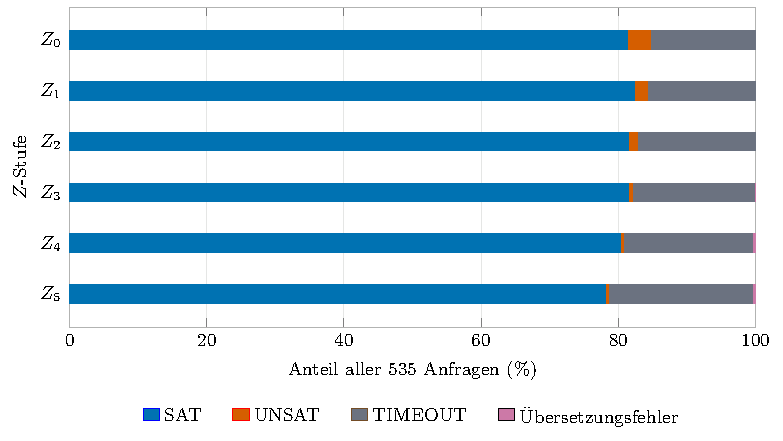
\includegraphics[width=\textwidth]
        {gfx/analysis_singleton_z_simple/statusverteilung.pdf}
    \caption[Ergebnisverteilung nach Größenstufe]{Relative
    Ergebnisverteilung der jeweils 535 vorgesehenen Anfragen. SAT
    bezeichnet nachgewiesene Unabhängigkeit, UNSAT nachgewiesene
    Abhängigkeit. TIMEOUTs und Übersetzungsfehler werden als eigene
    technische Kategorien ausgewiesen. Da hier der feste Nenner 535
    verwendet wird, unterscheiden sich die TIMEOUT-Anteile bei \(Z_3\) bis
    \(Z_5\) geringfügig von den um Übersetzungsfehler bereinigten Raten in
    Tabelle~\ref{tab:empirical-stable-z-status}.}
    \label{fig:empirical-stable-z-composition}
\end{figure}
\fi

Die bereinigte TIMEOUT-Rate nimmt von \(15{,}33\,\%\) bei \(Z_0\) auf
\(21{,}20\,\%\) bei \(Z_5\) zu. Dies entspricht einem Zuwachs von \(5{,}87\) Prozentpunkten. 
Die Rate steigt über alle sechs
Stufen hinweg schrittweise an. Demgegenüber sinkt der Anteil beobachteter
UNSAT-Ergebnisse unter den gelösten Anfragen von \(3{,}97\,\%\) auf
\(0{,}48\,\%\). Beide Verläufe sind in
Abbildung~\ref{fig:empirical-stable-z-rates} dargestellt.

\begin{figure}[H]
    \centering
    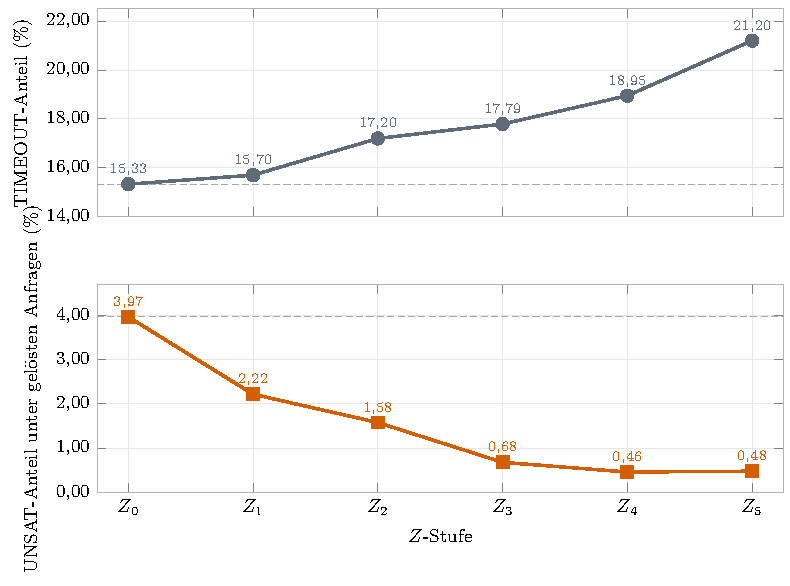
\includegraphics[width=\textwidth]
        {gfx/analysis_singleton_z_simple/ergebnistrends.pdf}
    \caption[Ergebnistrends nach Größenstufe]{TIMEOUT-Anteil unter den
    gültigen Solverläufen (oben) und UNSAT-Anteil unter den gelösten
    Anfragen (unten). Übersetzungsfehler sind aus der Berechnung
    ausgeschlossen. Die gestrichelte Linie markiert den Ausgangswert bei
    \(Z_0\).}
    \label{fig:empirical-stable-z-rates}
\end{figure}

Der Rückgang der beobachteten UNSAT-Ergebnisse darf nicht unmittelbar als
Rückgang der tatsächlichen Abhängigkeit interpretiert werden. Mit wachsendem
\(Z\) nimmt zugleich der Anteil der Anfragen zu, deren logischer Status
wegen eines TIMEOUTs unbekannt bleibt. Die Aussage beschränkt sich daher
darauf, dass unter den erfolgreich gelösten Anfragen seltener UNSAT
beobachtet wurde.

Für den Vorzeichentest können 105 Argumentationssysteme vollständig an
\(Z_0\) und \(Z_5\) verglichen werden. Zwei ABA2AF-Instanzen werden wegen
je eines Übersetzungsfehlers bei \(Z_5\) ausgeschlossen. Bei 95 der 105
Argumentationssysteme bleibt der TIMEOUT-Anteil unverändert. Zehn
Argumentationssysteme weisen bei \(Z_5\) einen höheren TIMEOUT-Anteil auf;
bei keinem nimmt er ab. Unter der Nullhypothese gleich wahrscheinlicher
Richtungen beträgt die Wahrscheinlichkeit für zehn gleichgerichtete
Änderungen im exakten zweiseitigen Vorzeichentest
\[
    p = 2\left(\frac{1}{2}\right)^{10}
      = 0{,}001953
      \approx 0{,}002.
\]
Bei einem vorab festgelegten Signifikanzniveau von
\(\alpha=0{,}05\) wird die Nullhypothese gleich wahrscheinlicher
Zu- und Abnahmen verworfen. Die Daten liefern damit Evidenz für einen
gerichteten Unterschied der beobachteten TIMEOUT-Anteile zwischen
\(Z_0\) und \(Z_5\).
Gleichzeitig zeigt
Abbildung~\ref{fig:empirical-stable-z-sign}, dass der Effekt nicht
gleichmäßig über alle Argumentationssysteme verteilt ist: Er konzentriert
sich auf zehn von 105 vollständig beobachteten Systemen
\((9{,}52\,\%)\), während der große Rest unverändert bleibt.

\begin{figure}[H]
    \centering
    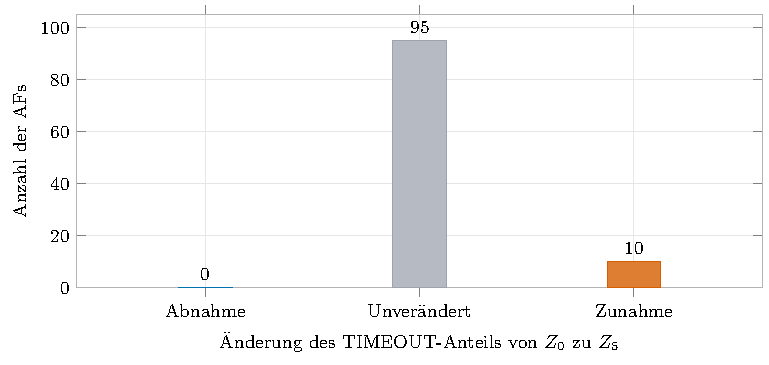
\includegraphics[width=\textwidth]
        {gfx/analysis_singleton_z_simple/vorzeichentest.pdf}
    \caption[AF-basierter Vergleich der kleinsten und größten Stufe]{Richtung der
    Änderung des TIMEOUT-Anteils zwischen \(Z_0\) und \(Z_5\) auf Ebene der
    Argumentationssysteme. Je System wurden die fünf Argumentpaare
    zusammengefasst. Dargestellt sind die 105 Systeme mit vollständig
    beobachteten Endpunkten. Zwei Systeme mit Übersetzungsfehler bei
    \(Z_5\) sind ausgeschlossen. Die 95 Bindungen werden berichtet, gehen
    aber nicht in den exakten Vorzeichentest ein.}
    \label{fig:empirical-stable-z-sign}
\end{figure}

\subsection{Unterschiede zwischen den Instanzfamilien}
\label{subsec:empirical-stable-z-families}

Die aggregierte Zunahme der TIMEOUT-Rate ist nicht für alle
Instanzfamilien gleichermaßen zu beobachten.
Abbildung~\ref{fig:empirical-stable-z-families} zeigt die TIMEOUT-Raten
getrennt nach Familie und \(Z\)-Stufe. Besonders deutlich ist der Effekt
für Barabási--Albert: Dort steigt die Rate von \(0\,\%\) bei \(Z_0\) auf
\(20\,\%\) bei \(Z_5\). Bei Planning2AF steigt sie bereits bis \(Z_2\) auf
\(33{,}3\,\%\) und bleibt anschließend auf diesem Niveau.

\begin{figure}[H]
    \centering
    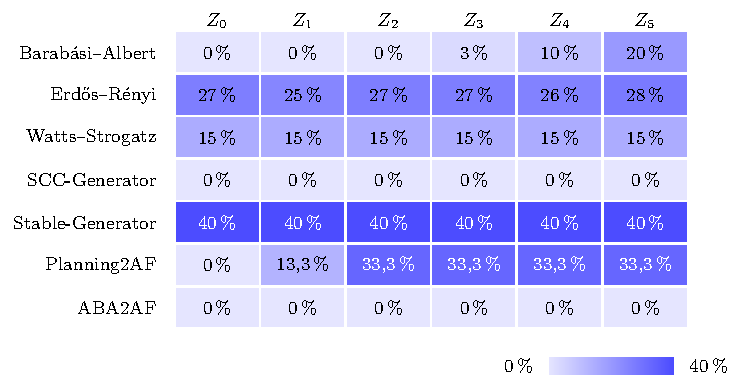
\includegraphics[width=\textwidth]
        {gfx/analysis_singleton_z_simple/familien-timeouts.pdf}
    \caption[TIMEOUT-Raten nach Instanzfamilie]{TIMEOUT-Rate in Prozent
    nach Instanzfamilie und \(Z\)-Stufe. Die Zellen sind auf eine
    Nachkommastelle gerundet. Übersetzungsfehler sind aus der Berechnung
    ausgeschlossen.}
    \label{fig:empirical-stable-z-families}
\end{figure}

Für Erdős--Rényi schwankt die Rate lediglich zwischen \(25\,\%\) und
\(28\,\%\). Beim Stable-Generator bleibt sie auf allen Stufen bei
\(40\,\%\), bei Watts--Strogatz bei \(15\,\%\). Für SCC-Generator und
ABA2AF treten keine TIMEOUTs auf. Von den zehn
Argumentationssystemen mit einer Zunahme im Endpunktvergleich stammen
sieben aus der Barabási--Albert-Familie, zwei aus Planning2AF und eines aus
Erdős--Rényi. Der allgemein beobachtete Trend lässt sich somit vor allem durch
Barabási--Albert und Planning2AF erklären. Eine allgemeine Aussage, nach
der ein größeres \(Z\) jedes Argumentationssystem erschwert, wäre somit aufgrund
der vorliegenden Daten nicht möglich.

\subsection{Solverlaufzeit}
\label{subsec:empirical-stable-z-runtime}

Neben der höheren TIMEOUT-Rate verschiebt sich auch der Anteil schnell
gelöster Anfragen. Abbildung~\ref{fig:empirical-stable-z-performance}
zeigt für jedes Zeitbudget \(t\), welcher Anteil aller 535 Anfragen einer
Stufe bis zu diesem Zeitpunkt gelöst wurde. Bei einem Budget von einer Sekunde
sinkt dieser Anteil von \(57{,}0\,\%\) bei \(Z_0\) auf \(45{,}2\,\%\) bei
\(Z_5\). Bei 100 Sekunden beträgt er \(81{,}3\,\%\) beziehungsweise
\(74{,}2\,\%\). Der Verlauf der Performanceprofile zeigt insgesamt: Mit
wachsendem \(Z\) wird ein kleinerer Anteil der Anfragen innerhalb desselben
Budgets gelöst.

\begin{figure}[H]
    \centering
    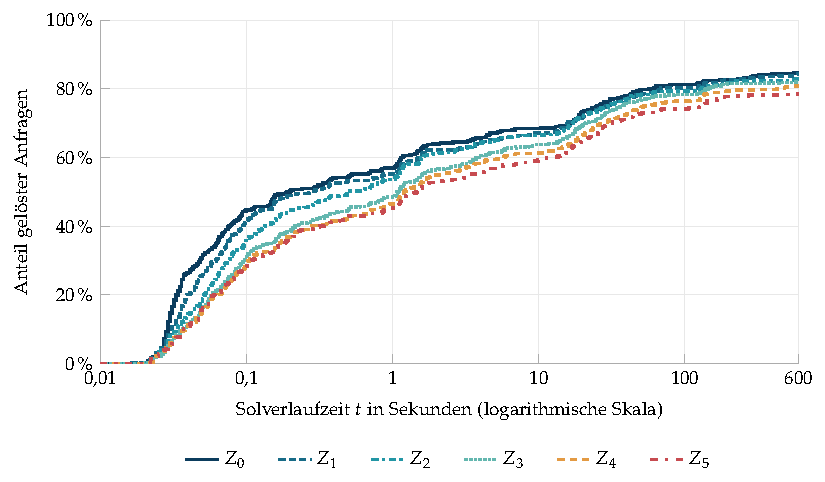
\includegraphics[width=\textwidth]
        {gfx/analysis_singleton_z_simple/performanceprofil.pdf}
    \caption[Performanceprofile nach Größe der Konditionierungsmenge]{Empirische
    Performanceprofile der sechs Größenstufen. Dargestellt ist für jedes
    Zeitbudget \(t\) der Anteil der je Stufe 535 vorgesehenen Anfragen, die
    bis \(t\) gelöst wurden. Die Zeitachse ist logarithmisch.}
    \label{fig:empirical-stable-z-performance}
\end{figure}

Dieser Unterschied lässt sich auch durch die Zeit bis zur Lösung der Hälfte
aller Anfragen ausdrücken. Bei \(Z_0\) sind \(50\,\%\) nach
\(0{,}198\) Sekunden gelöst, bei \(Z_5\) erst nach \(1{,}482\) Sekunden.
Das entspricht ungefähr dem Faktor \(7{,}5\).

\subsection{QBF-Größe und Erzeugungszeit}
\label{subsec:empirical-stable-z-qbf-overhead}

Die längeren Solverlaufzeiten können grundsätzlich zwei Ursachen haben. Zum
einen wächst mit \(Z\) die erzeugte QBF, sodass der Solver bereits rein
syntaktisch mehr Eingabedaten verarbeiten muss. Zum anderen verändert die
zusätzliche Konditionierung den logischen Aufbau der Formel und damit
möglicherweise die Schwierigkeit der internen Such- und
Propagationsschritte. Um beide Erklärungen deskriptiv gegenüberzustellen,
werden für jedes Argumentpaar die QBF-Kenngrößen einer Stufe mit den
Kenngrößen desselben Paars bei \(Z_0\) verglichen. Als Zusammenfassung wird
der Median der paarweisen Verhältnisse verwendet. Der Median ist für diesen
Vergleich geeignet, da einzelne ungewöhnlich lange Übersetzungs- oder
Solverläufe das Ergebnis weniger stark beeinflussen als bei einem
arithmetischen Mittel.

Für alle 3205 erfolgreich übersetzten Anfragen gelten exakt die Beziehungen
\[
    N_{\mathrm{var}} = 3n
    \qquad\text{und}\qquad
    N_{\mathrm{gate}} = 12n + 6|Z| + 16,
\]
wobei \(N_{\mathrm{var}}\) die Zahl der QBF-Variablen und
\(N_{\mathrm{gate}}\) die Zahl der QBF-Gatter bezeichnet. Die
Variablenzahl bleibt bei einer Änderung von \(Z\) folglich konstant. Jedes
zusätzliche Argument in \(Z\) fügt der verwendeten Kodierung dagegen genau
sechs Gatter hinzu.

\iffalse
Abbildung~\ref{fig:empirical-stable-z-qbf-overhead} zeigt, dass dieser
syntaktische Zuwachs über die Größenstufen annähernd linear verläuft. Bei
\(Z_5\) liegt die mediane Gatterzahl \(9{,}93\,\%\) und die mediane
QBF-Dateigröße \(6{,}53\,\%\) über dem jeweiligen Wert bei \(Z_0\). Die
mediane Übersetzungszeit nimmt demgegenüber lediglich um \(1{,}00\,\%\)
zu. Der größere Umfang der Kodierung verursacht somit nur einen geringen
zusätzlichen Aufwand bei der QBF-Erzeugung.

\begin{figure}[H]
    \centering
    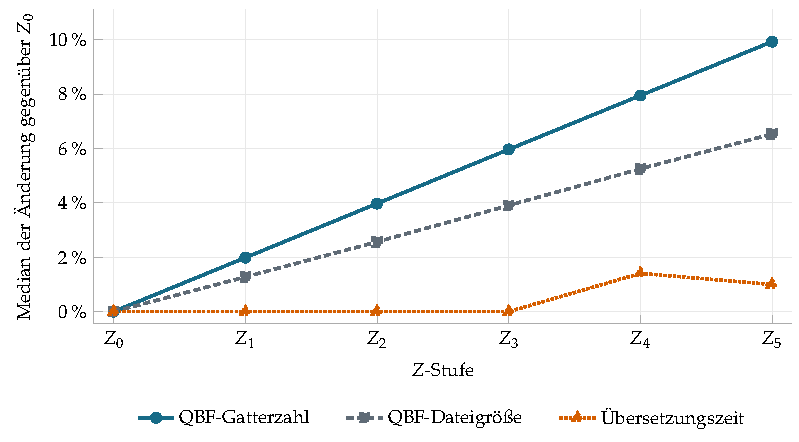
\includegraphics[width=\textwidth]
        {gfx/analysis_singleton_z_simple/qbf-overhead.pdf}
    \caption[QBF-Größe und Übersetzungszeit nach Größenstufe]{Median der
    paarweisen relativen Änderungen von QBF-Gatterzahl, QBF-Dateigröße und
    Übersetzungszeit gegenüber \(Z_0\). Verglichen wird jeweils dasselbe
    Argumentpaar; Paare mit einem Übersetzungsfehler am Vergleichsendpunkt
    werden ausgeschlossen. Es gehen 535 Paare bei \(Z_1\) und \(Z_2\), 534
    bei \(Z_3\) sowie 533 bei \(Z_4\) und \(Z_5\) ein. Die konstante
    QBF-Variablenzahl ist nicht dargestellt.}
    \label{fig:empirical-stable-z-qbf-overhead}
\end{figure}
\fi

Gegen eine ausschließlich durch die syntaktische Größe verursachte
Verlangsamung spricht insbesondere der Vergleich der Instanzfamilien in
Abbildung~\ref{fig:empirical-stable-z-qbf-runtime}. Die mediane
Gatterzahl steigt in jeder Familie von \(Z_0\) nach \(Z_5\) um ungefähr
den Faktor \(1{,}10\). Die mediane Solverlaufzeit erhöht sich bei
Barabási--Albert jedoch um den Faktor \(6{,}79\) und bei Planning2AF um
den Faktor \(5{,}04\). In den übrigen Familien liegt der Laufzeitfaktor
trotz eines nahezu identischen Gatterzuwachses nur zwischen \(1{,}00\)
und \(1{,}10\). Der Umfang der QBF allein ist daher keine hinreichende
Erklärung für die beobachtete Verlangsamung.

\begin{figure}[H]
    \centering
    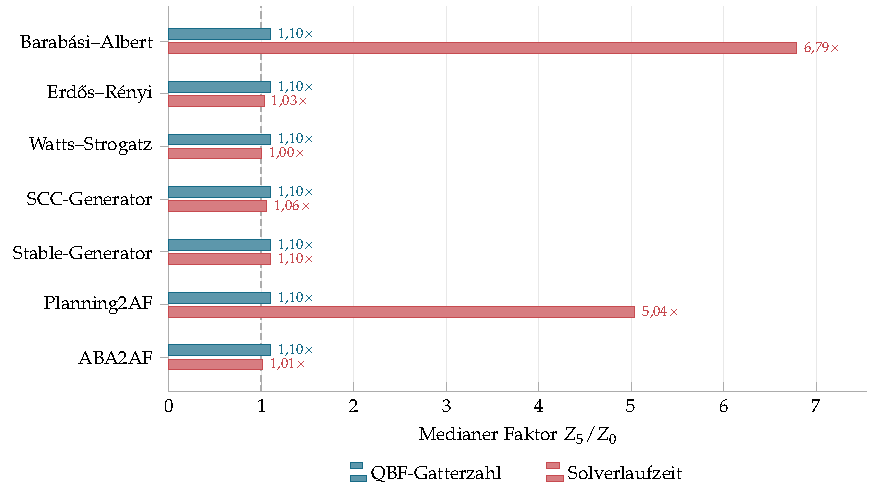
\includegraphics[width=\textwidth]
        {gfx/analysis_singleton_z_simple/qbf-runtime-vergleich.pdf}
    \caption[QBF-Größe und Solverlaufzeit nach Instanzfamilie]{Median der
    paarweisen Faktoren von \(Z_5\) gegenüber \(Z_0\), getrennt nach
    Instanzfamilie. Für die Gatterzahl werden Paare mit erfolgreicher
    Übersetzung an beiden Endpunkten berücksichtigt. Der Laufzeitfaktor
    umfasst nur Paare, die an beiden Endpunkten gelöst wurden. Die
    Laufzeitfaktoren beruhen in der dargestellten Reihenfolge auf 80, 71,
    85, 30, 60, 20 und 73 Paaren.}
    \label{fig:empirical-stable-z-qbf-runtime}
\end{figure}

Die Ergebnisse sprechen damit dafür, dass vor allem die durch ein größeres
\(Z\) veränderte logische Struktur die solverseitige Schwierigkeit erhöht,
während das moderate syntaktische Wachstum nur einen kleineren Anteil
erklärt. Eine eindeutige kausale Trennung ist mit dem vorliegenden
Versuchsaufbau jedoch nicht möglich, da eine größere Konditionierungsmenge 
gleichzeitig den Umfang und den logischen Inhalt der QBF verändert. 

\subsection{Einordnung und Einschränkungen}
\label{subsec:empirical-stable-z-limitations}

Die Auswertung zeigt im Durchschnitt einen klaren Zusammenhang zwischen einem
größeren \(Z\) und einer schwierigeren praktischen Lösung: für feste Zeitbudgets 
werden weniger Anfragen gelöst. Der
Vorzeichentest liefert zusätzliche Evidenz für die gerichtete Zunahme der
TIMEOUT-Rate zwischen \(Z_0\) und \(Z_5\). Die Auswertung der einzelnen Instanzfamilien
relativiert dieses Ergebnis jedoch: Die Erhöhung des TIMEOUT-Anteils im
Endpunktvergleich betrifft nur einen kleinen Teil der
Argumentationssysteme und wird hauptsächlich durch zwei Instanzfamilien
getragen.

Bei der Interpretation sind vier Einschränkungen wesentlich. Erstens sind
die Mengen \(Z_k\) unabhängig gezogen und nicht geschachtelt. Verglichen
werden daher zufällige Mengen unterschiedlicher Größe und nicht die
schrittweise Erweiterung einer festen Menge. Zweitens existiert je Paar
und Größenstufe nur eine Ziehung von \(Z_k\). Der Einfluss der Größe kann
somit nicht vollständig vom Einfluss der konkreten Zusammensetzung
getrennt werden. Drittens verdecken TIMEOUTs den logischen SAT- oder
UNSAT-Status. Insbesondere erlaubt der beobachtete Rückgang des
UNSAT-Anteils keine Aussage über den unbekannten Status der nicht gelösten
Anfragen. Viertens besteht die Datengrundlage aus einer Auswahl von
Benchmarkinstanzen. Eine uneingeschränkte Verallgemeinerung auf beliebige
andere Argumentationssysteme ist deshalb nicht gerechtfertigt.

Insgesamt stützen die Daten die Aussage, dass größere
Konditionierungsmengen die Lösung der Stable-QBFs im untersuchten
Benchmark erschweren können. Dieser Effekt ist in der Ergebnisverteilung
und in den Lösungsquoten sichtbar, fällt aber stark
familienabhängig aus und ist nicht bei jedem Argumentationssystem zu
beobachten. Der geringe Zuwachs von QBF-Größe und Übersetzungszeit reicht
als alleinige Erklärung für die ausgeprägten Laufzeiteffekte in den
Barabási--Albert- und Planning2AF-Instanzen nicht aus.
